\themaD
\graphicspath{{../../S27_Frequence_et_moyenne/Images/}}

\chapter{Fréquence\\et moyenne}
\label{S27}


%%%%%%%%%%%%%%%%%%%%%%%%%%%%%%
%%%%%%%%%%%%%%%%%%%%%%%%%%%%%%
\begin{autoeval}
   \small
   \begin{enumerate}
      \item Il calcule des effectifs et des fréquences.
      \item Il calcule et interprète la moyenne de données.
   \end{enumerate}
\end{autoeval}

\begin{prerequis}
   \begin{itemize}
      \item Effectifs, fréquences.
      \item Indicateur de position : moyenne.
      \item[\com] Calculer des effectifs, des fréquences.
      \item[\com] Calculer et interpréter des indicateurs de position
   \end{itemize}
\end{prerequis}

\vfill

\begin{debat}[Débat : les statistiques]
   Les premiers textes écrits retrouvés sur les {\bf statistiques} étaient des recensements de bétail. On attribue souvent l'introduction du terme {\bf statistique} au professeur {\it Achenwall}, qui aurait, en 1746, créé le mot {\it Statistik}, dérivé de l'allemand {\it Staatskunde}. \\
   Même si cette branche des mathématiques est récente, elle fait partie des notions les plus utilisées actuellement et les plus gros consommateurs de statistiques sont les assureurs (risques d'accidents, de maladie des assurés), les médecins (épidémiologie), les démographes (populations et leur dynamique), les économistes (emploi, conjoncture économique), les météorologues\dots
   \begin{center}
      \textcolor{B1}{\psset{unit=0.8}
      \begin{pspicture}(0,-0.25)(5,3.5)
         \it\small
          \rput{10}(0,0){maximum}
         \rput{20}(1.5,1){moyenne}
         \rput{-10}(3,0){minimum}
         \rput{-20}(4.5,1){fréquence}
         \rput{30}(0.5,2){médiane}
         \rput{-30}(2,3){mode}
         \rput{40}(3.5,2){écart-type}
         \rput{-25}(5,3){histogramme}
         \rput(-0.5,3){quartiles}
      \end{pspicture}}
   \end{center}
   \bigskip
   \begin{cadre}[B2][J4]
      \begin{center}
         Vidéo : \href{https://www.yout-ube.com/watch?v=aOX0pIwBCvw}{\bf Chocolat, corrélation et moustache de chat}, chaîne YouTube {\it La statistique expliquée à mon chat}.
      \end{center}
   \end{cadre}
\end{debat}


%%%%%%%%%%%%%%%%%%%%%%%%%%%%%%%%%%
%%%%%%%%%%%%%%%%%%%%%%%%%%%%%%%%%
\activites

\begin{activite}[Pourquoi étudier les statistiques ?]
   {\bf Objectif :} avoir un regard critique envers les chiffres et les informations que l'on nous donne.
   \begin{QCM}
      Pourquoi étudier les statistiques ? Entre autres pour savoir démêler le vrai du faux dans les publicités, les journaux\dots{} Pour chaque ligne du tableau suivant, discuter de ce que vous pouvez déduire immédiatement des données brutes que l'on vous donne, puis étudier ce que l'on pourrait ajouter dans la colonne de droite. \\
      Cela change-t-il votre opinion ? \medskip
      \begin{center}
         {\small
         \hautab{2}
         \begin{CLtableau}{0.85\linewidth}{3}{c}
            \hline
            & Ce qu'on vous dit & Ce qu'on oublie de vous dire \\
            \hline
            1 & Au loto, 100\,\% des gagnants ont tenté leur chance. & Le pourcentage de gagnants par rapport au nombre total de joueurs. \\
            \hline
            2 & M. Truc a largement remporté les élections avec 60\,\% des suffrages. & Le taux d’abstention a été de 50\,\%. \\
            \hline
            4 & En 1995, au Brésil, 16\,\% des enfants étaient au travail et au Guatemala : 15,9\,\%. & Le Brésil compte 170 millions d’habitants et le Guatemala 12,7 millions d’habitants.  \\
            \hline
            5 & La température annuelle moyenne de Moscou est de 5 degrés. \newline Que prendrez-vous dans vos valises ? & Quel mois partez-vous ? \\
            \hline
            6 & Il y a en France environ 200\,000 licenciés à la Fédération française de tir à l'arc. En Chine, il y en a 1\,500\,000. \newline C'est un sport beaucoup plus pratiqué en Chine qu'en France. & La France compte 60\,000\,000 habitants et la Chine 1\,200\,000\,000 habitants. \\
            \hline
            7 & C’est un vendredi noir à la Bourse ! Forte chute des valeurs ! & Et si on prenait une autre échelle ? \\
             & \footnotesize
                \psset{yunit=0.7}
                \begin{pspicture}(-1,-0.5)(5,5.5)
                   \psset{linecolor=lightgray}
                   \multido{\r=0+0.5,\n=3760+10}{11}{\psline(0,\r)(5,\r) \rput(-0.5,\r){\n}}  
                   \multido{\n=0+1}{6}{\rput(\n,0){|}}
                   \psline[linecolor=black](0.5,4.5)(1,3.5)(1.5,4)(2,3.75)(2.5,3)(3,2.75)(3.5,1.5)(4,1.75)(4.5,0.5)
               \end{pspicture}
              & \footnotesize
                \psset{yunit=0.7}
                \begin{pspicture}(-1,-0.5)(5,5.5)
                   \psset{linecolor=lightgray}
                   \multido{\r=0+0.5,\n=3500+50}{11}{\psline(0,\r)(5,\r) \rput(-0.5,\r){\n}}  
                   \multido{\n=0+1}{6}{\rput(\n,0){|}}
                   \psline[linecolor=black](0.5,3.5)(1,3.3)(1.5,3.4)(2,3.35)(2.5,3.2)(3,3.15)(3.5,2.9)(4,2.95)(4.5,2.7)
               \end{pspicture} \\
            \hline
         \end{CLtableau}}
      \end{center} \medskip
      Ce que nous apprend ce tableau c'est que l'on peut faire dire n'importe quoi aux chiffres, et ainsi déformer la réalité, donc il faut toujours avoir à l'esprit que les résultats d'une étude statistique peuvent être fortement biaisés. \\
   \end{QCM}
   \vfill\hfill{\footnotesize\it Source : d'après \href{http://maths.spip.ac-rouen.fr/IMG/pdf/Statistiques.pdf}{\og Les statistiques dans les nouveaux programmes du cycle central \fg}, académie de Rouen}
\end{activite}


%%%%%%%%%%%%%%%%%%%%%%%%%%%%%%%
%%%%%%%%%%%%%%%%%%%%%%%%%%%%%%%
\cours 

%%%%%%%%%%%%%%%%
\section{Effectifs et fréquences}

On demande aux élèves d'une classe de 5\up{e} quel est son loisir principal et combien de temps il passe à le pratiquer. On obtient les résultats suivants arrondis à l'heure près :
\begin{center}
   {\footnotesize
   \begin{ttableau}{0.95\linewidth}{7}
      \hline
      Judo \hfill 6 & Gymnastique \hfill 4 & Hand-ball \hfill 5 & Hand-ball \hfill 4 & Tennis \hfill 2 & Karaté \hfill 2 & Équitation \hfill 1 \\
      G.R.S. \hfill 10 & Hand-ball \hfill 5 & Natation \hfill 2 & Lego\textregistered \hfill 3 & Badminton \hfill 14 & Football \hfill 8 & Danse \hfill 2 \\
      Taekwondo \hfill 7 & Lecture \hfill 3 & Boxe \hfill 2 & Danse \hfill 2 & Courir \hfill 6 & Taekwondo \hfill 6 & Musique \hfill 7 \\
       Hand-ball \hfill 3 & Piano \hfill 4 & Vidéos \hfill 10 & Dessiner \hfill 10 & Lecture \hfill 30 & & \\
      \hline
   \end{ttableau}}
\end{center}

 \begin{definition}
   \begin{itemize}
      \item L'{\bf effectif} d'une donnée est le nombre de fois qu'elle apparaît ; si on fait la somme des effectifs on obtient l'{\bf effectif total}.
      \item La {\bf fréquence} d'une donnée est le quotient de l'effectif de cette donnée par l'effectif total. Elle s'exprime par un nombre décimal entre compris entre 0 et 1 ou en pourcentage. \\ [-9mm]
   \end{itemize}
\end{definition}
 
\begin{exemple*1}
   Tableau des effectifs et des fréquences. \\ [2mm]
      {\small 
      \Stat[Tableau,CouleurTab=FondTableaux,Largeur=7mm,Donnee=Durée (h),PrecisionF=1,Total,Stretch=1.2,Frequence]{1/1,2/6,3/3,4/3,5/2,6/3,7/2,8/1,10/3,14/1,30/1}}
   \ \\ [-6mm]
\end{exemple*1}

\medskip

On peut également faire un regroupement par classes, ce qui rend l'étude moins précise, mais ce qui permet d'avoir une vision plus globale.

\begin{exemple*1}
   Tableau des effectifs par classes d'amplitude 5 heures.
   \begin{center}
      {\small
      \hautab{1.2}
      \begin{CLtableau}{0.9\linewidth}{8}{c}
         \hline       
         Durée (h) & \; $]~0~;~5~]$ & $]~5~;~10~]$ & $]~10~;~15~]$ & $]~15~;~20~]$ & $]~20~;~25~]$ & $]~25~;~30~]$ & Total \\
         \hline
         Effectif & \quad\, 15 & \quad\, 9 & \quad\, 1 & \quad\, 0 & \quad\, 0 & \quad\, 1 & \quad\, 26 \\
         \hline
      \end{CLtableau}}
   \end{center}
   \vspace*{-7mm}
\end{exemple*1}


%%%%%%%%%%%%%%%%
\section{Moyenne arithmétique}

\begin{definition}
   La \textbf{moyenne} d'une série est égale au quotient de la somme des données par l'effectif total.
\end{definition}

\begin{methode*1}[Calcul d'une moyenne pondérée]
   Pour obtenir la somme des données dans le cas où les données sont pondérées (effectif $\neq1)$ :
   \begin{itemize}
      \item on multiplie chaque effectif par sa donnée, puis on fait la somme ;
      \item lorsque les données sont présentées par classes, on choisit le centre de la classe comme donnée que l'on multiplie par l'effectif, puis on fait la somme.
   \end{itemize}
   Puis on divise cette somme par l'effectif total.
   \exercice
      Quel est le temps moyen passé sur le loisir principal de la classe de 5\up{e} ? Faire le calcul avec le tableau simple $(\overline{m})$ et le tableau par classes $(\overline{m_c})$.
   \correction
      \small $\overline{m_c} =\dfrac{15\times2,5+9\times7,5+1\times12,5+0\times17,5+0\times22,5+1\times27,5}{26} =\dfrac{145}{26} \approx5,6$. \\ [2mm] 
      {\footnotesize $\overline{m} =\dfrac{1\times1+6\times2+3\times3+3\times4+2\times5+3\times6+2\times7+1\times8+3\times10+1\times14+1\times30}{26} =\dfrac{158}{26} \approx6,1$.}
\end{methode*1}


%%%%%%%%%%%%%%%%%%%%%%%%%%%%%%%%%%
%%%%%%%%%%%%%%%%%%%%%%%%%%%%%%%%%%
\exercicesbase

\begin{colonne*exercice}

\begin{exercice} %1
   Le diagramme en bâtons ci-dessous représente le temps de trajet journalier en minutes de 36 personnes travaillant dans l'entreprise Kadubol.
   \begin{center}
      {\footnotesize  
   \Stat[Graphique,Grille,Unitex=0.12,Unitey=0.4,Pasx=5,EpaisseurBatons=5,Donnee=,Effectif=Nombre de personnes,LectureFine,Tiret,CouleurDefaut=Gray]{5/1,10/3,15/2,20/2,25/4,30/7,35/5,40/4,45/3,50/2,55/0,60/3} \\ [-2mm]
   \hspace*{50mm} Temps en minutes}
   \end{center}  
   \vspace*{-5mm}
   \begin{enumerate}
      \item
      \begin{enumerate}
         \item Construire le tableau d'effectifs et de fréquences récapitulant toutes ces valeurs.
         \item Calculer la moyenne
      \end{enumerate}
      \item
      \begin{enumerate}
         \item Construire le tableau des effectifs en les regroupant par classes d'amplitude 15 minutes en commençant par la classe ]~0~;~15~].
         \item Calculer la moyenne en utilisant la répartition par classes. Le résultat obtenu est-il le même que lors du calcul précédent ? Pourquoi ? Est-il plus fiable ?
      \end{enumerate}
   \end{enumerate}
\end{exercice}

\begin{corrige}
   \ \\ [-5mm]
   \begin{enumerate}
      \item
      \begin{enumerate}
         \item Tableau des effectifs et des fréquences en \% \\ \smallskip
         {\footnotesize
         \hautab{1.3}
         \begin{ltableau}{\linewidth}{12}
            \hline
            5 & 10 & 15 & 20 & 25 & 30 & 35 & 40 & 45 & 50 & 55 & 60 \\
            \hline
            1 & 3 & 2 & 2 & 4 & 7 & 5 & 4 & 3 & 2 & 0 & 3 \\
            \hline
            \!2,8 & \!8,3 & \!5,6 & \!5,6 & \!\!11,1 & \!\!19,4 & \!\!13,9 & \!\!11,1 & \!8,3 & \!5,6 & 0 & \!8,3 \\
            \hline
         \end{ltableau}}
         \item $\overline{m} =(1\times5+3\times10+2\times15+2\times20+4\times25+7\times30+5\times35+4\times40+3\times45+2\times50+0\times55+3\times60)\div36 =1\,165\div36 \approx32,4$. \\
         {\blue La moyenne est de \umin{32,4}}.
      \end{enumerate}   
      \setcounter{enumi}{1}
      \item
      \begin{enumerate}
      \item Tableau des effectifs par classes. \\ \smallskip
      {\small
      \hautab{1.3}
      \begin{lctableau}{0.9\linewidth}{5}
         \hline
         Durée & $]\,0\,;\,15\,]$ & $]\,15\,;\,30\,]$ & $]\,30\,;\,45\,]$ & $]\,45\,;\,60\,]$ \\
         \hline
         Eff.& \quad 6 & \quad 13 & \quad 12 & \quad 5 \\
         \hline
      \end{lctableau}}
      \item $\overline{m} =(6\times7,5+13\times22,5+12\times37,5+5\times52,5)\div36 \approx 29,2$. {\blue La moyenne est de \umin{29,2}}. \\
         Ce résultat est différent de celui trouvé dans la question précédente car on perd en précision, puisqu'on ne s'occupe plus de la valeur exacte, mais de l'appartenance à un intervalle plus grand.
      \end{enumerate}
   \end{enumerate}
\end{corrige}

\smallskip


\begin{exercice} %2
   Le tableau suivant résume les résultats obtenus par une classe lors d'une évaluation.
   \begin{center}
   {\small
      \Stat[Tableau,CouleurTab=FondTableaux,Largeur=1.5mm,Donnee=N,Effectif=E,Stretch=1.2]{3/1,5/2,6/1,7/3,8/3,9/5,10/6,11/4,12/2,13/1,14/2,17/2,18/1}}
   \end{center}
   \begin{enumerate}
      \item Combien y a-t-il d'élèves dans cette classe ?
      \item Compléter le tableau par les fréquences.
      \item Quel est le pourcentage d'élèves ayant obtenu une note inférieure ou égale à 8 ?
      \item Déterminer la moyenne de la série de notes.
      \item Cette évaluation était la quatrième de la période. \\
         Toutes les évaluations ont le même coefficient et jusqu'alors Bastien avait 9 de moyenne ; après ce devoir, il a 9,5 de moyenne. Quelle note a-t-il obtenue à ce devoir ? 
   \end{enumerate}
\end{exercice}

\begin{corrige}
   \ \\ [-5mm]
   \begin{enumerate}
      \item $1+2+1+3+3+5+6+4+2+1+2+2+1 =33$. Donc, {\blue il y a 33 élèves dans cette classe}.
      \item Tableau des fréquences en \%. \\ \smallskip
      {\small
      \hautab{1.3}
      \begin{lctableau}{\linewidth}{14}
         \hline
         N & 3 & 5 & 6 & 7 & 8 & 9 & \!10 & \!11 & \!12 & \!13 & \!14 & \!17 & \!18 \\
         \hline
         E & 1 & 2 & 1 & 3 & 3 & 5 & 6 & 4 & 2 & 1 & 2 & 2 & 1 \\
         \hline
         F & 3 & 6 & 3 & 9 & 9 & \!\!15 & \!\!18 & \!\!12 & 6 & 3 & 6 & 6 & 3 \\
         \hline
     \end{lctableau}}
      \item $p =\dfrac{1+2+1+3+3}{33}\times100 =\dfrac{10}{33}\times100 \approx30,3$. \\ [1.5mm]
      Environ {\blue 30,3\,\% des élèves} ont obtenu une note inférieure ou égale à 8. \smallskip
      \item $\overline{m} =(1\times3+2\times5+1\times6+3\times7+3\times8+5\times9+6\times10+4\times11+2\times12+1\times13+2\times14+2\times17+1\times18)\div33 =330\div33 =10$. \\
      {\blue La moyenne est de 10}.
      \item La moyenne après le 4\up{e} devoir est de 9,5 donc, la somme de ses notes est de $4\times9,5 =38$. \\
         La somme des trois premiers devoirs était de $3\times9 =27$.  Or, $38-27 =11$ donc  : \\
         {\blue Bastien a obtenu 11} au dernier devoir.
  \end{enumerate}
\end{corrige}

\smallskip


\begin{exercice} %3
   Quatre-vingts archers d'un club de tir à l'arc A ont participé à un championnat. Le nombre de points obtenus par chaque archer du club est donné par le diagramme ci-dessous.
   \begin{center}
      {\footnotesize      
      \Stat[Graphique,Grille,Unitex=0.65,Unitey=0.25,Pasx1,EpaisseurBatons=5,Donnee=,Effectif=Nombre d'archers,LectureFine,Tiret,CouleurDefaut=Gray]{0/0,1/0,2/5,3/9,5/8,6/12,7/14,8/6,9/8,10/18} \\ [-2mm]
   \hspace*{50mm} Nombre de points}
   \end{center}
   \vspace*{-10mm}
   \begin{enumerate}
      \item 
      \begin{enumerate}
         \item Combien d'archers ont gagné exactement six points lors de ce championnat ?
         \item Combien d'archers ont gagné trois points ou plus lors de ce championnat ?
      \end{enumerate}
      \item Le club de tir à l'arc B a aussi participé à ce championnat. Voici quelques données :
      \begin{itemize}
         \item Le score moyen des archers lors du championnat est 7 points.
         \item Le score moyen des dix meilleurs archers lors du championnat est 9,9 points. \\ [-10mm]
      \end{itemize}
      \begin{enumerate}
         \item Comparer les résultats des deux clubs selon leurs scores moyens.
         \item Comparer les résultats des deux clubs selon les scores de leurs dix meilleurs archers.
      \end{enumerate}
   \end{enumerate}
\end{exercice}

\begin{corrige}
   \ \\ [-5mm]
   \begin{enumerate}
      \item
      \begin{enumerate}
         \item {\blue 12 d'archers} ont gagné six points.
         \item 5 archers ont obtenu 2 points. Or, $80-5 =75$ \\
            donc, {\blue 75 ont gagné trois points ou plus}.
      \end{enumerate}
      \setcounter{enumi}{1}
      \item 
      \begin{enumerate}
         \item Score moyen des archers du club A : \\
            $\overline{m} =(5\times2+9\times3+8\times5+12\times6+14\times7+6\times8+8\times9+18\times10)\div80 =547\div80 =6,8375$. \\
            Or, le score moyen du club B est de 7 points donc, c'est {\blue le club B} qui a le score moyen le plus élevé.
         \item Les 10 meilleurs archers du club A ont marqué 10 points alors que la moyenne des 10 meilleurs archers du club B est de 9,9 points donc, c'est {\blue le club A} qui possède les dix meilleurs résultats.
      \end{enumerate}
   \end{enumerate}
\end{corrige}

\end{colonne*exercice}

\smallskip


\begin{exercice} %4
   Ce tableau présente les températures moyennes mensuelles à Tours en 2019.
   \begin{center}
      
      \Stat[Tableau,Qualitatif,CouleurTab=FondTableaux,Donnee=Mois,Effectif=Température (\udeg{}C),Largeur=6mm] {J/4.4,F/7.8,M/9.6,A/11.2,M/13.4,J/19.4,J/22.6,A/20.5,S/17.9,O/14.4,N/8.2,D/7.8}
   \end{center}
   \begin{enumerate}
      \item D'après le tableau, quelle a été la température moyenne à Tours en novembre 2019 ?
      \item Vérifier que la température moyenne annuelle est \udegc{13,1}.
      \item La température moyenne annuelle à Tours en 2009 était de \udegc{11,9}. Le pourcentage d'augmentation entre 2009 et 2019, arrondi à l'unité, est-il de :  7\,\% ; 10\,\%  ou 13\,\%  ? Justifier la réponse.
   \end{enumerate}
\end{exercice}

\begin{corrige}
   \ \\ [-5mm]
      \begin{enumerate}
      \item La température moyenne à Tours en novembre 2019 a été de {\blue \udegc{8,2}}.
      \item $(4,4+7,8+9,6+11,2+13,4+19,4+22,6+20,5+17,9+ 14,4+8,2+7,8)\div12$ \\
         $=157,2\div12 =13,1$. {\blue La température moyenne annuelle à Tours en 2019 était de \udegc{13,1}}. \smallskip
         \item \textcolor{G1}{$\bullet$} Calcul avec 7\,\% : $\dfrac{7}{100}\times\udegc{11,9} =\udegc{0,833}$. \\ [1mm]
            $\udegc{11,9}+\udegc{0,833} =\udegc{12,733} \neq\udegc{13,1}$. \\ [1mm]
            \textcolor{G1}{$\bullet$} Calcul avec  10\,\% : $\dfrac{10}{100}\times\udegc{11,9} =\udegc{1,19}$. \\ [1mm]
            $\udegc{11,9}+\udegc{1,19} =\udegc{13,09} \approx\udegc{13,1}$. \\
           {\blue Le pourcentage d'augmentation de la température entre 2009 et 2019 a été d'environ 10\,\%}.
   \end{enumerate}
\end{corrige}


%%%%%%%%%%%%%%%%%%%%%%%%%%%%%%%%%%%
%%%%%%%%%%%%%%%%%%%%%%%%%%%%%%%%%%%
\Recreation

\begin{enigme}[Cryptographie]
   La cryptographie est l'ensemble des techniques permettant de protéger une communication au moyen d'un code graphique secret. Parmi elles, on retrouve la méthode de substitution monoalphabétique : les lettres du texte à coder sont remplacées par d’autres lettres tel que  deux lettres différentes sont codées de façons différentes et que la même lettre est toujours codée de la même façon. \\
   \begin{minipage}{12cm}
      Le savant arabe {\it Al-Kindi}  (Abu Yūsuf Ya'qūb ibn'Ishāq as-Sabbāh al-Kindī) met au point, au 9\up{e} siècle, une technique appelée analyse des fréquences afin de déchiffrer les messages secrets. Elle repose sur la comparaison entre les fréquences d'apparition des lettres dans un message crypté à partir d'une langue connue avec la fréquence d'apparition moyenne des lettres dans cette langue. \\ [3mm]
      En français, par exemple, on a la répartition suivante représentée par \\
      un diagramme en bâtons, basée sur l'analyse de milliers de romans. 
   \end{minipage}
   \qquad
   \begin{minipage}{4cm}
      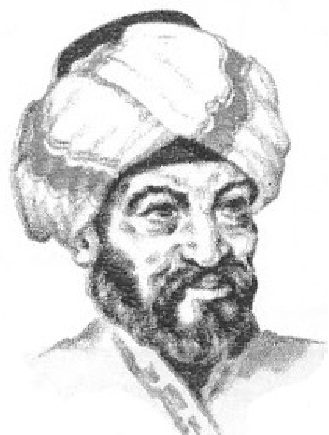
\includegraphics[width=3.5cm]{Al-kindi}
   \end{minipage}
   \begin{center}
      {\footnotesize
   
      \Stat[Graphique,Qualitatif,Donnee=,Effectif=Fréquence d'apparition de la lettre (\%),Grille,Unitex=0.6,Unitey=0.33,EpaisseurBatons=4,LectureFine,Tiret,CouleurDefaut=Gray]{A/7.68,B/0.8,C/3.32,D/3.6,E/17.76,F/1.06,G/1.1,H/0.64,I/7.23,J/0.19,K/0,L/5.89,M/2.72,N/7.61,O/5.34,P/3.24,Q/1.34,R/6.81,S/8.23,T/7.3,U/6.05,V/1.27,W/0,X/0.54,Y/0.21,Z/0.07}}
   \end{center}  
   Ainsi, il y a des chances que la lettre la plus fréquente du message crypté soit la traduction de la lettre E, très fréquente en français. Les lettres très peu fréquentes ou absentes dans un message auront tendance à être les traductions de K ou W, par exemple. \\

   Calculer la fréquence de chaque lettre du message codé ci-dessous (on pourra représenter les résultats dans un tableau). En observant les correspondances entre le diagramme en bâton et votre tableau, décoder le message.
   
   \begin{center}
      \fbox{
         \begin{minipage}{13cm}
            \ \\ [-1mm]
            BKSMAMZCZMTFY \; KF \; OKATOCFZ \; ZHKY \; CYZIAMKIYKUKFZ \; AK \; UKYYCLK \; ATOK \; RTIY \; CRKP \; BHCFADM \; IF \; XCY \; OKAMYMB \; RKHY \; SC \; YTSIZMTF \; BMFCSK \; OCFY \; AKZZK \; CAZMRMZK \; UCZDKUCZMGIK \; VHCRT
         \end{minipage}}
   \end{center}

   \vfill
   
   {\it Pour retrouver la correspondance de chaque lettre, on pourra tout d'abord retrouver la lettre la plus fréquente qui correspond à un E, puis chercher les mots courts de 2 lettres par exemple.
   
   \vfill
   
      \hspace*{8cm}\rotatedown{Spoiler : l'un des mots du message décrypté est \og message \fg.}}
\end{enigme}

\begin{corrige}
   On obtient les effectifs et fréquences suivants : \\
{\footnotesize
\begin{Ltableau}{\linewidth}{9}{c}
   \hline
   A & B & C & D & E & F & G & H & I \\
   \hline
   9 & 4 & 13 & 2 & 0 & 9 & 1 & 3 & 6 \\
   \hline
   6,67 & 2,96 & 9,63 & 1,48 & 0 & 6,67 & 0,74 & 2,22 & 4,44 \\
   \hline
   C & F & A & H & & N & Q & R & U \\
   \hline
\end{Ltableau}

\begin{Ltableau}{\linewidth}{9}{c}
   \hline
   J & K & L & M & N & O & P & Q & R \\
   \hline
   0 & 20 & 1 & 12 & 0 & 5 & 1 & 0 & 4 \\
   \hline
   0 & 14,81 & 0,74 & 8,89 & 0 & 3,7 & 0,74 & 0 & 2,95 \\
   \hline
   & E & G & I & & D & Z & & V \\
   \hline
\end{Ltableau}

\begin{Ltableau}{\linewidth}{8}{c}
   \hline
   S & T & U & V & W & X & Y & Z \\
   \hline
   4 & 6 & 4 & 1 & 0 & 1 & 12 & 13 \\
   \hline
   2,96 & 4,44 & 2,96 & 0,74 & 0 & 0,74 & 8,89 & 9,63 \\
   \hline
   L & O & M & B & & P & S & T \\
   \hline
\end{Ltableau}}

En analysant ces données, on peut décrypter le message suivant : \og Félicitations : en décodant très astucieusement ce message codé, vous avez franchi un pas décisif vers la solution finale dans cette activité mathématique. Bravo ! \fg
\end{corrige}
